% !TEX root = ../main.tex

\subsection{Spiral Winding}

In order to test the possible progenitor distribution of our estimated galaxy pitch angles, we repeatedly perform an Anderson-Darling test over each draw present in the MCMC trace, resulting in a distribution of Anderson-Darling statistics. We will refer to this test as the \textit{marginalized Anderson-Darling test}.

We perform the marginalized Anderson-Darling test on a distribution uniform in $\cot\phi$ between the limits present in \citet{2019arXiv190910291P} ($1.00 < \cot\phi < 4.75$, or roughly $11.9 < \phi < 45.0$). The resulting distribution of Anderson-Darling statistics can be seen in Figure \ref{fig:ad-cot-test}. We observe that we reject the null hypothesis at the 1\% level for only 92\% of the possible realizations of galaxy pitch angle. Therefore we cannot unilaterally reject winding of the kind described by \citet{2019arXiv190910291P}, though .

\begin{figure*}
  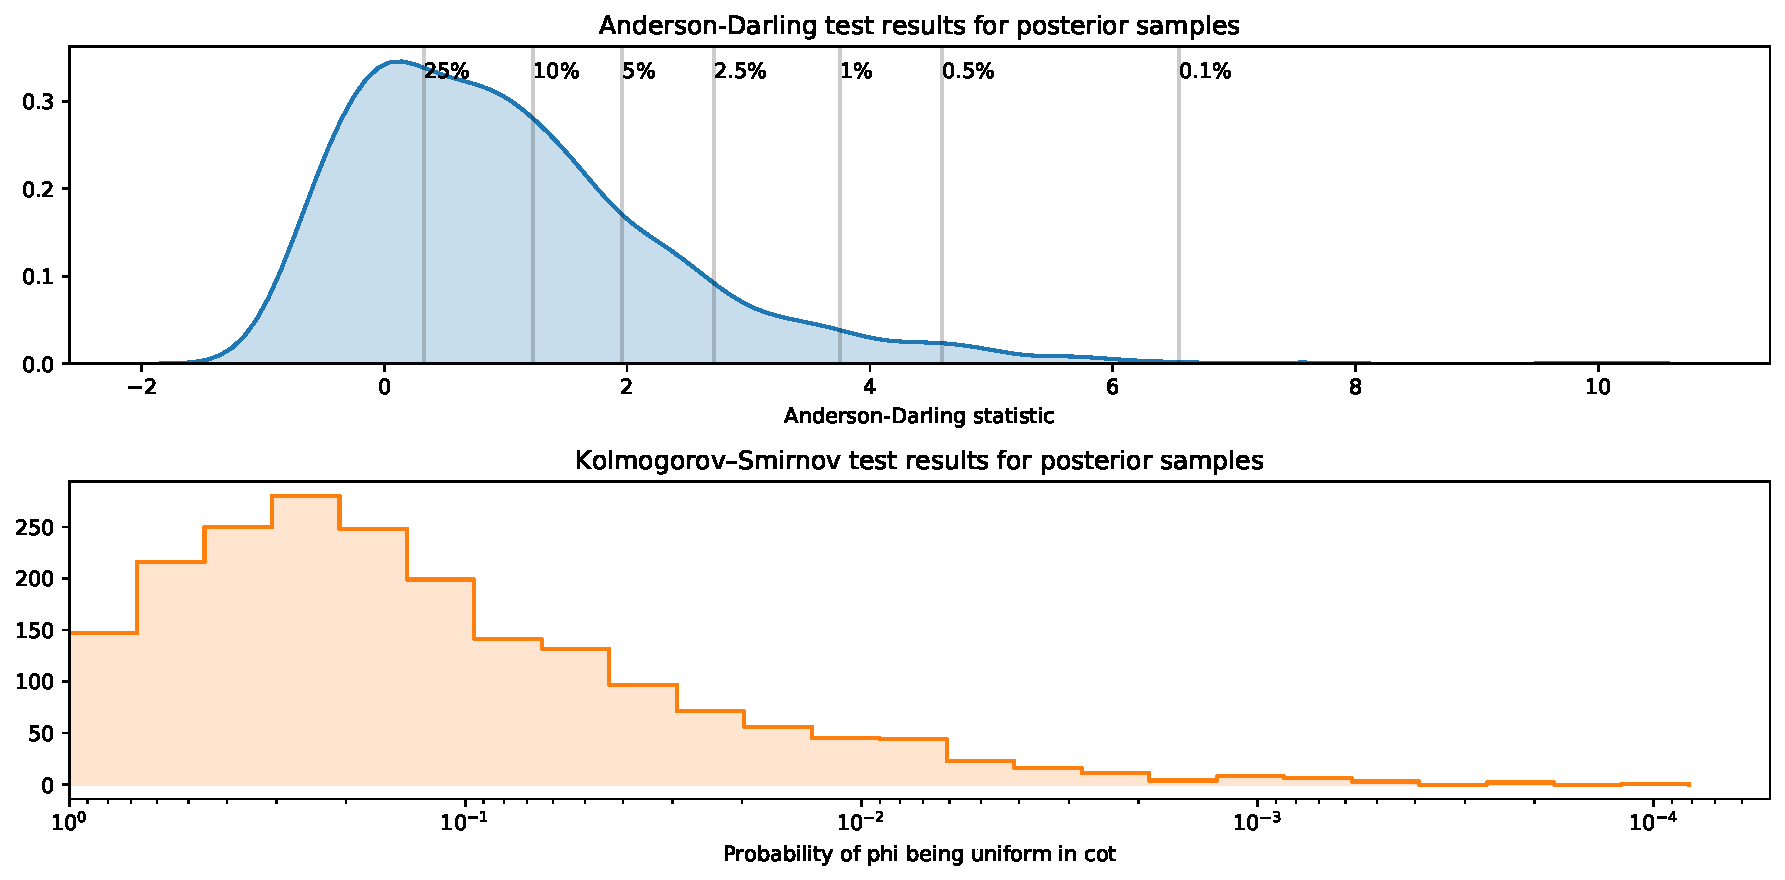
\includegraphics[width=17.7cm]{plots/cot_uniform_marginalized_tests.pdf}
  \caption{The results of a marginalized Anderson-Darling test (top panel), with confidence intervals shown, and marginalized Kolmogorov-Smirnov test p-values (lower panel).}
  \label{fig:ad-cot-test}
\end{figure*}

\subsection{Dependence of pitch angle on Galaxy Morphology}
\label{section:morphology_comparision}
\subsubsection{Pitch angle vs. Bulge size}
We see no correlation between galaxy pitch angle derived from the \textit{hierarchial normal model} and GZ2's \textit{pbulge}, which is widely viewed as a good measure of bulge size.



\subsubsection{Pitch angle vs. Bar Strength}
We see no correlation between galaxy pitch angle derived from the \textit{hierarchial normal model} and GZ2's \textit{pbar}, which is widely viewed as a good measure of bar strength, and therefore a measure of the torque applied on the disc gas.

A marginalized Anderson-Darling test does not find that the samples were drawn from different distributions (statistic of -0.91).
